%% abtex2-modelo-artigo.tex, v-1.9.7 laurocesar
%% Copyright 2012-2018 by abnTeX2 group at http://www.abntex.net.br/ 
%%
%% This work may be distributed and/or modified under the
%% conditions of the LaTeX Project Public License, either version 1.3
%% of this license or (at your option) any later version.
%% The latest version of this license is in
%%   http://www.latex-project.org/lppl.txt
%% and version 1.3 or later is part of all distributions of LaTeX
%% version 2005/12/01 or later.
%%
%% This work has the LPPL maintenance status `maintained'.
%% 
%% The Current Maintainer of this work is the abnTeX2 team, led
%% by Lauro César Araujo. Further information are available on 
%% http://www.abntex.net.br/
%%
%% This work consists of the files abntex2-modelo-artigo.tex and
%% abntex2-modelo-references.bib
%%

% ------------------------------------------------------------------------
% ------------------------------------------------------------------------
% abnTeX2: Modelo de Artigo Acadêmico em conformidade com
% ABNT NBR 6022:2018: Informação e documentação - Artigo em publicação 
% periódica científica - Apresentação
% ------------------------------------------------------------------------
% ------------------------------------------------------------------------

\documentclass[
	% -- opções da classe memoir --
	article,			% indica que é um artigo acadêmico
	11pt,				% tamanho da fonte
	oneside,			% para impressão apenas no recto. Oposto a twoside
	a4paper,			% tamanho do papel. 
	% -- opções da classe abntex2 --
	chapter=TITLE,		% títulos de capítulos convertidos em letras maiúsculas
	section=TITLE,		% títulos de seções convertidos em letras maiúsculas
	subsection=TITLE,	% títulos de subseções convertidos em letras maiúsculas
	subsubsection=TITLE, % títulos de subsubseções convertidos em letras maiúsculas
	% -- opções do pacote babel --
	english,			% idioma adicional para hifenização
	brazil,				% o último idioma é o principal do documento
	sumario=tradicional
	]{ifrs-farr-artigo-abntex2}


% ---
% PACOTES
% ---

% ---
% Pacotes fundamentais 
% ---
\usepackage{lmodern}			% Usa a fonte Latin Modern
\usepackage[T1]{fontenc}		% Selecao de codigos de fonte.
\usepackage[utf8]{inputenc}		% Codificacao do documento (conversão automática dos acentos)
\usepackage{indentfirst}		% Indenta o primeiro parágrafo de cada seção.
\usepackage{nomencl} 			% Lista de simbolos
\usepackage{color}				% Controle das cores
\usepackage{graphicx}			% Inclusão de gráficos
\usepackage{microtype} 			% para melhorias de justificação
% ---
		
% ---
% Pacotes adicionais, usados apenas no âmbito do Modelo Canônico do abnteX2
% ---
\usepackage{lipsum}				% para geração de dummy text
% ---
		
% ---
% Pacotes de citações
% ---
\usepackage[brazilian,hyperpageref]{backref}	 % Paginas com as citações na bibl
\usepackage[alf]{abntex2cite}	% Citações padrão ABNT
% ---

% ---
% Configurações do pacote backref
% Usado sem a opção hyperpageref de backref
\renewcommand{\backrefpagesname}{Citado na(s) página(s):~}
% Texto padrão antes do número das páginas
\renewcommand{\backref}{}
% Define os textos da citação
\renewcommand*{\backrefalt}[4]{
	\ifcase #1 %
		Nenhuma citação no texto.%
	\or
		Citado na página #2.%
	\else
		Citado #1 vezes nas páginas #2.%
	\fi}%
% ---

% --- Informações de dados para CAPA e FOLHA DE ROSTO ---
\titulo{Modelo Artigo Científico}
%\tituloestrangeiro{}

\curso{Curso 01/2019}

\autor{Discente: Alice\footnote{alice@fake.com}}

\orientador{ Bob\footnote{bob@fake.edu.br}}

\instituicao{Instituto Federal de Educação Ciência e Tecnologia do Rio Grande do Sul}
\local{Campus Farroupilha}

\data{\today}
% ---

% ---
% Configurações de aparência do PDF final

% alterando o aspecto da cor azul
\definecolor{blue}{RGB}{41,5,195}

% informações do PDF
\makeatletter
\hypersetup{
     	%pagebackref=true,
		pdftitle={\@title}, 
		pdfauthor={\@author},
    	pdfsubject={Modelo de artigo científico com abnTeX2},
	    pdfcreator={LaTeX with abnTeX2},
		pdfkeywords={abnt}{latex}{abntex}{abntex2}{atigo científico}, 
		colorlinks=true,       		% false: boxed links; true: colored links
    	linkcolor=blue,          	% color of internal links
    	citecolor=blue,        		% color of links to bibliography
    	filecolor=magenta,      		% color of file links
		urlcolor=blue,
		bookmarksdepth=4
}
\makeatother
% --- 

% ---
% compila o indice
% ---
\makeindex
% ---

% ---
% Altera as margens padrões
% ---
\setlrmarginsandblock{3cm}{2cm}{*}
\setulmarginsandblock{3cm}{2cm}{*}
\checkandfixthelayout
% ---

% --- 
% Espaçamentos entre linhas e parágrafos 
% --- 

% O tamanho do parágrafo é dado por:
\setlength{\parindent}{1.3cm}

% Controle do espaçamento entre um parágrafo e outro:
\setlength{\parskip}{0.2cm}  % tente também \onelineskip

% Espaçamento simples
\SingleSpacing

\setlength{\ABNTEXcitacaorecuo}{1.8cm}
% ----
% Início do documento
% ----
\begin{document}
% Seleciona o idioma do documento (conforme pacotes do babel)
%\selectlanguage{english}
\selectlanguage{brazil}

% Retira espaço extra obsoleto entre as frases.
\frenchspacing 

% ----------------------------------------------------------
% ELEMENTOS PRÉ-TEXTUAIS
% ----------------------------------------------------------

%---
%
% Se desejar escrever o artigo em duas colunas, descomente a linha abaixo
% e a linha com o texto ``FIM DE ARTIGO EM DUAS COLUNAS''.
% \twocolumn[    		% INICIO DE ARTIGO EM DUAS COLUNAS
%
%---

% página de titulo principal (obrigatório)
%\maketitle
\imprimircapa
% titulo em outro idioma (opcional)
\hrule
% resumo em português
\renewcommand{\resumoname}{}
\begin{resumo}
\textbf{Resumo:}Modelo baseado no \citeonline{abntex}. Adição de característica pertinentes a tipos de documentos (artigos, monografias...) devem ser realizadas na classe LaTex correspondente (.cls). Adição de características generalizáveis a diversas classes de documentos, devem ser realizadas em \textit{packages} (.sty).
 
 \vspace{\onelineskip}
 
 \noindent
 \textbf{Palavras-chave}: palavra1. palavra2. palavra3.
\end{resumo}
\hrule

% resumo em inglês
\renewcommand{\resumoname}{}
\begin{resumoumacoluna}
 \begin{otherlanguage*}{english}
   \textbf{Abstract:} According to ABNT NBR 6022:2018, an abstract in foreign language is optional.

   \vspace{\onelineskip}
 
   \noindent
   \textbf{Keywords}: word1. word2.
 \end{otherlanguage*}  
\end{resumoumacoluna}
\hrule

% ]  				% FIM DE ARTIGO EM DUAS COLUNAS
% ---

%\begin{center}\smaller
%\textbf{Data de submissão e aprovação}: elemento obrigatório. Indicar dia, mês e ano
%
%\textbf{Identificação e disponibilidade}: elemento opcional. Pode ser indicado 
%o endereço eletrônico, DOI, suportes e outras informações relativas ao acesso.
%\end{center}

% ----------------------------------------------------------
% ELEMENTOS TEXTUAIS
% ----------------------------------------------------------
\textual

% ----------------------------------------------------------
% Introdução
% ----------------------------------------------------------

\section{Dicas LaTex}

Instalação corretor ortográfico no Texmaker:
\url{https://github.com/abntex/abntex2/wiki/Texmaker}.

Exemplo de referência ao fim: Integer sollicitudin nisi vel pellentesque posuere. Aenean porttitor et purus ac rutrum \cite{pribeream2013}.

Exemplo de citação na linha: segundo \citeonline{fidBond}, este é só um exemplo.

Segundo \apudonline{evMoeda}{ratti2001comercio},isto é só para mostrar apud.

Segundo \apudonline{btcBub}{irratBub}, isto é só para mostrar apud com et. al. .
\newpage
Exemplo de colocação de figura na Figura \ref{fig_config_edit}.

\begin{figure}[htb]
	\caption{\label{fig_config_edit}Esta é um rótulo de figura.}
	\begin{center}
	    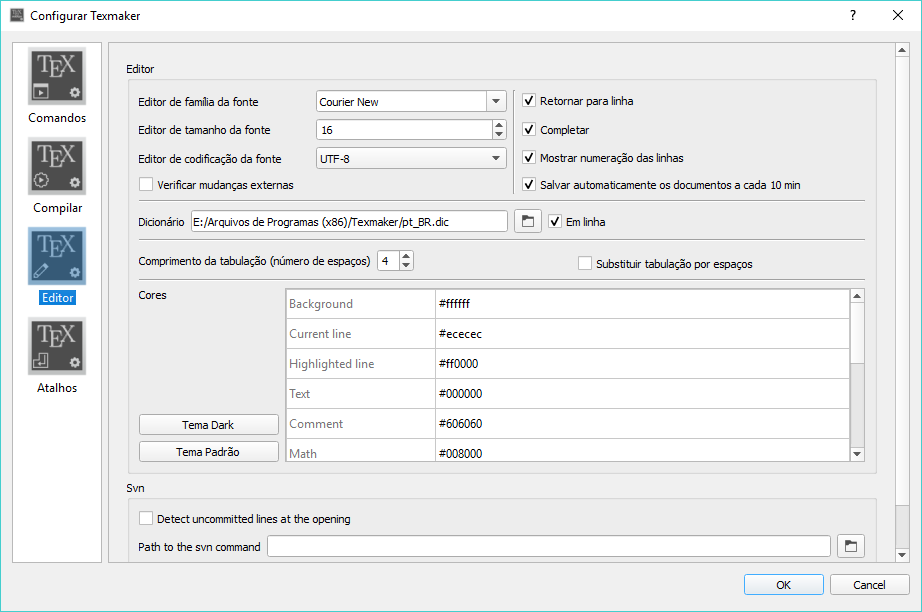
\includegraphics[scale=0.4]{figuras/config_editor_texmaker.png}
	\end{center}
	\legend{Fonte: \citeonline{verGe}.}
\end{figure}


Outro exemplo: Figura \ref{fig_config_comand}:

\begin{figure}[h]
	\caption{\label{fig_config_comand}Este é outro rótulo de figura.}
	\begin{center}
	    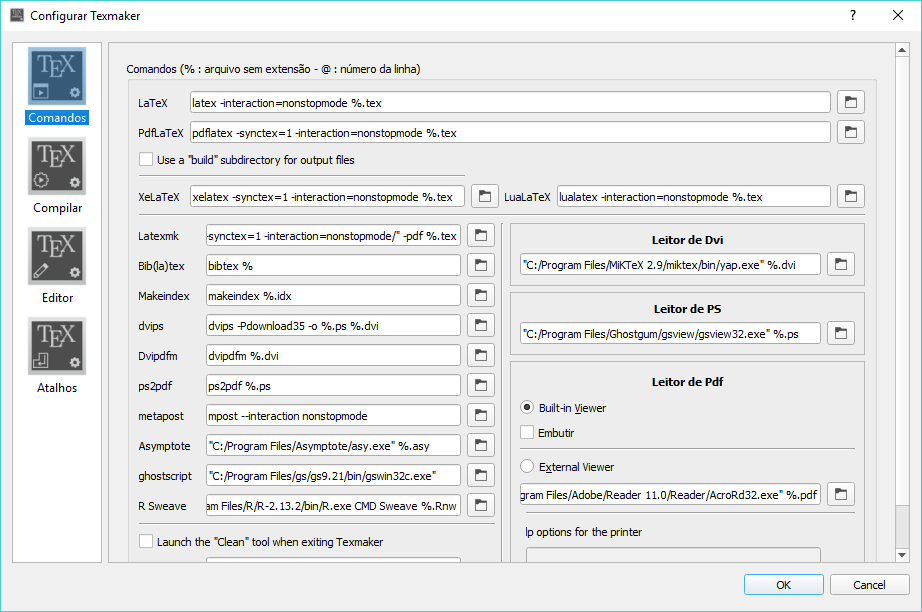
\includegraphics[scale=0.5]{figuras/config_comandos_texmaker.png}
	\end{center}
	\legend{Fonte: o autor.}
\end{figure}

\newpage
\section{Introdução}
\begin{citacao}
"Integer sollicitudin nisi vel pellentesque posuere. Aenean porttitor et purus ac rutrum.\cite{costa2009}"
\end{citacao}

Da onde?

Quando?

Porque?

\subsection{Objetivo Geral}
Que a estrutura deste modelo seja usada apenas como referência, não como uma forma imutável. Que esta estrutura melhore com sugestões de quem usa-la. Que quem use, possa focar na solução sendo pesquisada, não na formatação do documento.

\subsection{Objetivos Específicos}
\begin{itemize}
    \item Pesquisar e analisar.
	\item Implementar.
	\item Explorar.
	\item Realizar.
	\item Utilizar.
	\item Fazer uso.
\end{itemize}

\section{Revisão Bibliográfica}
Buscar validar o caráter de ineditismo da proposta.

Quem já fez algo parecido?

O que era? Como funcionou?

Que resultados teve?
\begin{citacao}
"Cuidar para não ser técnico, descrever a solução, não citar detalhes da implementação. Falar de maneira didática para não necessitar de referencial já aqui."
\end{citacao}
\section{Referencial Teórico}

Para falar da solução o leitor tem de ter referencial para garantir um mínimo entendimento.

\textbf{Brevemente}, como funciona o que foi usado para resolver?
 
  
\begin{table}[htb]
  \begin{center}
    \label{tabela-oneway}
    \begin{tabular}{|c|c|c|c|c|c|c|c|c|c|c|c|c|c|c|c|c|}
      \hline
      $x$ & 1 & 2 & 3 & 4 & 5 & 6 & 7 & 8 & 9 & 10 & 11 & 12 & 13 & 14 & 15 & 16 \\
      $f(x)$ & 3 & 9 & 10 & 13 & 5 & 15 & 11 & 16 & 14 & 8 & 7 & 4 & 12 & 2 & 6 & 1 \\
      \hline
    \end{tabular}
  \end{center}
\end{table}

\section{Desenvolvimento}
Foco maior daqui para frente.
\subsection{Materiais e Método}
Por quais meios?

\subsubsection{Método}
Qualitativo, quantitativo, pesquisa...
\subsubsection{Material 1}
O que é o que foi usado para resolver?

Com que finalidade metodológica?

\section{Conclusão}
\section{Resultados e Discussão}
Como ficou o que foi feito para resolução do problema da pesquisa?

Apresentar explicando, sem interpretar os resultados.

% ---
% Finaliza a parte no bookmark do PDF, para que se inicie o bookmark na raiz
% ---
\bookmarksetup{startatroot}% 
% ---

% ---
% Conclusão
% ---
\section{Considerações Finais}
Se chegou aos objetivos?

Interpretar os resultados.

Recomendar ou não mais pesquisa na solução proposta.

\newpage
% ----------------------------------------------------------
% ELEMENTOS PÓS-TEXTUAIS
% ----------------------------------------------------------
\postextual

% ----------------------------------------------------------
% Referências bibliográficas
% ----------------------------------------------------------
\bibliography{ifrs-farr-modelo-references}
% ----------------------------------------------------------
% Glossário
% ----------------------------------------------------------
%
% Há diversas soluções prontas para glossário em LaTeX. 
% Consulte o manual do abnTeX2 para obter sugestões.
%
%\glossary

% ----------------------------------------------------------
% Apêndices
% ----------------------------------------------------------

% ---
% Inicia os apêndices
% ---
%\begin{apendicesenv}
%
%% ----------------------------------------------------------
%\chapter{Nullam elementum urna vel imperdiet sodales elit ipsum pharetra ligula
%ac pretium ante justo a nulla curabitur tristique arcu eu metus}
%% ----------------------------------------------------------
%\lipsum[55-56]
%
%\end{apendicesenv}
%% ---
%
%% ----------------------------------------------------------
%% Anexos
%% ----------------------------------------------------------
%\cftinserthook{toc}{AAA}
%% ---
%% Inicia os anexos
%% ---
%%\anexos
%\begin{anexosenv}
%
%% ---
%\chapter{Cras non urna sed feugiat cum sociis natoque penatibus et magnis dis
%parturient montes nascetur ridiculus mus}
%% ---
%
%\lipsum[31]
%
%\end{anexosenv}
%
%% ----------------------------------------------------------
%% Agradecimentos
%% ----------------------------------------------------------
%
%\section*{Agradecimentos}
%Texto sucinto aprovado pelo periódico em que será publicado. Último 
%elemento pós-textual.

\end{document}
